\newcommand{\mytt}[1]{\texttt{#1}}
\newcommand{\comprehension}[3]{\{ \; #1; \; #2; \; #3 \; \}}
\newcommand{\aggregate}[6]{[\; #1 \Rightarrow #2; \; #3; \; #4; \; #5; \; #6 \;]}
\newcommand{\codemargin}[0]{0.7cm} 

LM is a forward-chaining linear logic programming language that allows logical
facts to be asserted and retracted in a structured fashion.  A LM program can be
seen as a graph of nodes, where each node contains a database of logical facts.
The program is written as a set of inference rules that apply over the logical
facts of a node. When rules are applied, facts are asserted or retracted from
the node database.

LM rules have the form \mytt{a(X), b(Y) -o c(X, Y)} and can be read as follows:
if fact \mytt{a(X)} and fact \mytt{b(Y)} exist in the database then fact
\mytt{c(X, Y)} is added to the database. The expression \mytt{a(X), b(Y)} is
called the \emph{body} of the rule and \mytt{c(X, Y)} is called the \emph{head}
of the rule.  A fact is a predicate, e.g., \mytt{a}, \mytt{b} or \mytt{c}, and
its associated tuple of values, e.g., the concrete values of \mytt{X} and
\mytt{Y}. Since LM uses linear logic as its foundation, we distinguish between
\emph{linear} and \emph{persistent facts}. Linear facts are consumed (deleted)
during the process of deriving a rule, while persistent facts are not.  Program
execution starts by adding the initial facts (called the axioms) to the
database. Next, rules are recursively applied and the database is updated by
adding new facts or deleting facts used during rule derivation.  When no more
rules are applicable, the program terminates. Rules have a defined priority
(their position in the source file) and higher priority rules are fired first.
If a new fact is derived and there is a set of applicable rules to be fired, the
higher priority rule is selected before the others.

To make these ideas concrete, Fig.~\ref{code:shortest_path_program} presents a
simple example for the single source shortest path~(SSSP) program.  The program
computes the shortest distance from node \mytt{@1} to all other nodes in the
graph.  The SSSP program starts (lines 1-3) with the declaration of the
predicates.  Predicates specify the facts used in the program. The first
predicate, \mytt{edge}, is a persistent predicate that describes the
relationship between the nodes of the graph, where the third argument represents
the weight of the edge (the \mytt{route} modifier informs the compiler that the
\mytt{edge} predicate determines the structure of the graph).  The predicates
\mytt{shortest} and \mytt{relax} are specified as linear facts and thus are
deleted when deriving new facts.  In the example, every node has a
\mytt{shortest} fact that can be improved with new \mytt{relax} facts.  Lines
5-9 declare the axioms of the program: \mytt{edge} facts describe the graph;
\mytt{shortest(A, +00, [])} is the initial shortest distance (infinity) for all
nodes; and \mytt{relax(@1, 0, [@1])} starts the algorithm by setting the
distance from \mytt{@1} to \mytt{@1} to be 0.

\begin{topfig}
\begin{Verbatim}[numbers=left,xleftmargin=\codemargin,fontsize=\scriptsize]
type route edge(node, node, int).
type linear shortest(node, int, list int).
type linear relax(node, int, list int).

!edge(@1, @2, 3). !edge(@1, @3, 1).
!edge(@3, @2, 1). !edge(@3, @4, 5).
!edge(@2, @4, 1).
shortest(A, +00, []).
relax(@1, 0, [@1]).

shortest(A, D1, P1), D1 > D2, relax(A, D2, P2)
   -o shortest(A, D2, P2),
      {B, W | !edge(A, B, W) |
         relax(B, D2 + W, P2 ++ [B])}.

shortest(A, D1, P1), D1 <= D2, relax(A, D2, P2)
   -o shortest(A, D1, P1).
\end{Verbatim}
\caption{Single Source Shortest Path program code.}
\label{code:shortest_path_program}
\end{topfig}

The first rule of the program (lines 11-14) reads as following: if the current
\mytt{shortest} path \mytt{P1} with distance \mytt{D1} is larger than a new
\texttt{relax} path with distance \mytt{D2}, then replace the current shortest
path with \mytt{D2}, delete the new \mytt{relax} and propagate new paths to
the neighbors (lines 13-14) using a \emph{comprehension}.  The comprehension
iterates over the edges of node \mytt{A} and derives a new \mytt{relax} fact for
each node \mytt{B} with the distance \mytt{D2 + W}, where \mytt{W} is the weight
of the edge.

The second rule of the program (lines 16-17) is read as following: if the
current shortest distance \mytt{D1} is shorter than a new \texttt{relax}
distance \mytt{D2}, then delete the new \mytt{relax} fact and keep the current
shortest path.

Figure~\ref{fig:shortest_path_program} shows a graphical representation of the
application of the SSSP program rules.

\begin{figure}[ht]
\begin{center}
  \subfloat[]{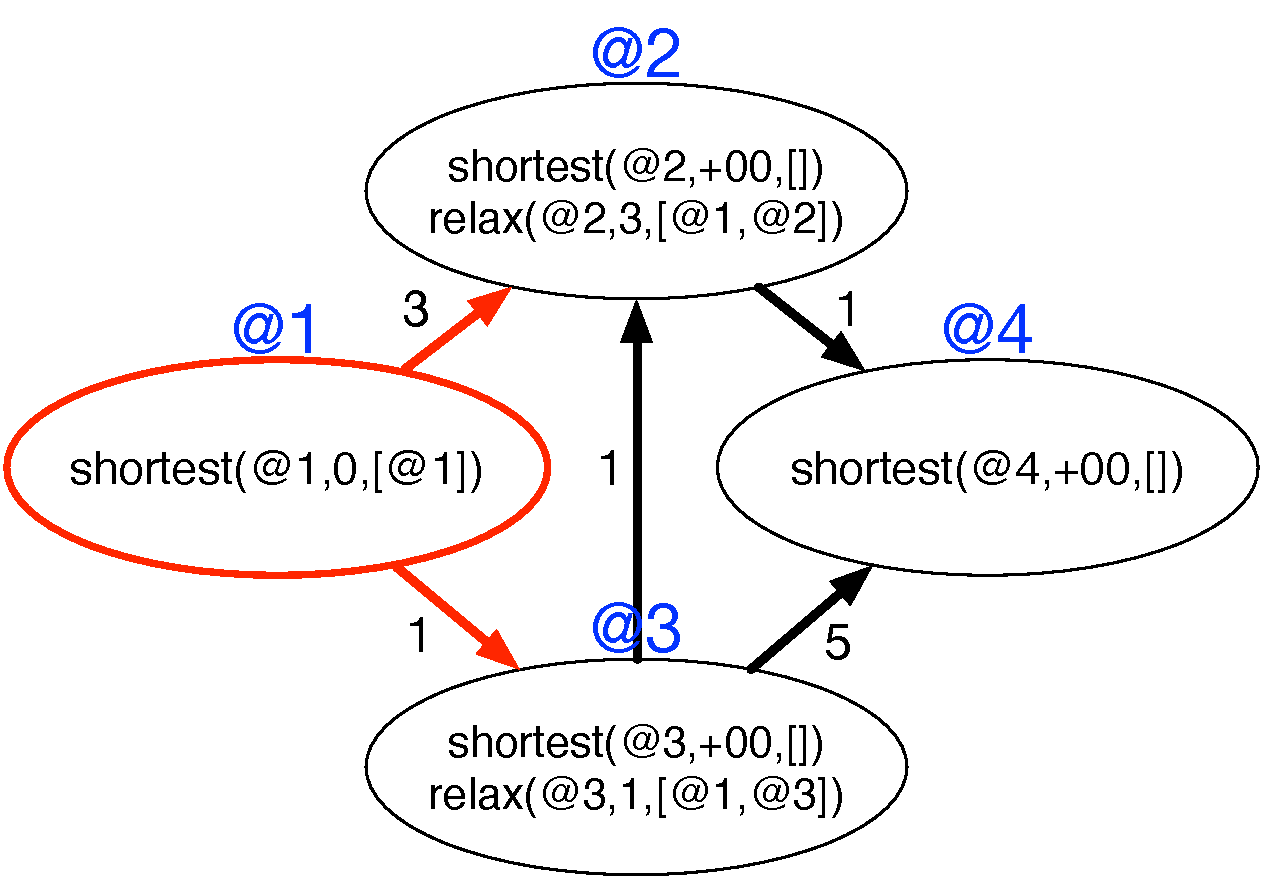
\includegraphics[width=0.32\textwidth]{figures/shortest2}}
  \hspace{0.02cm}
  \subfloat[]{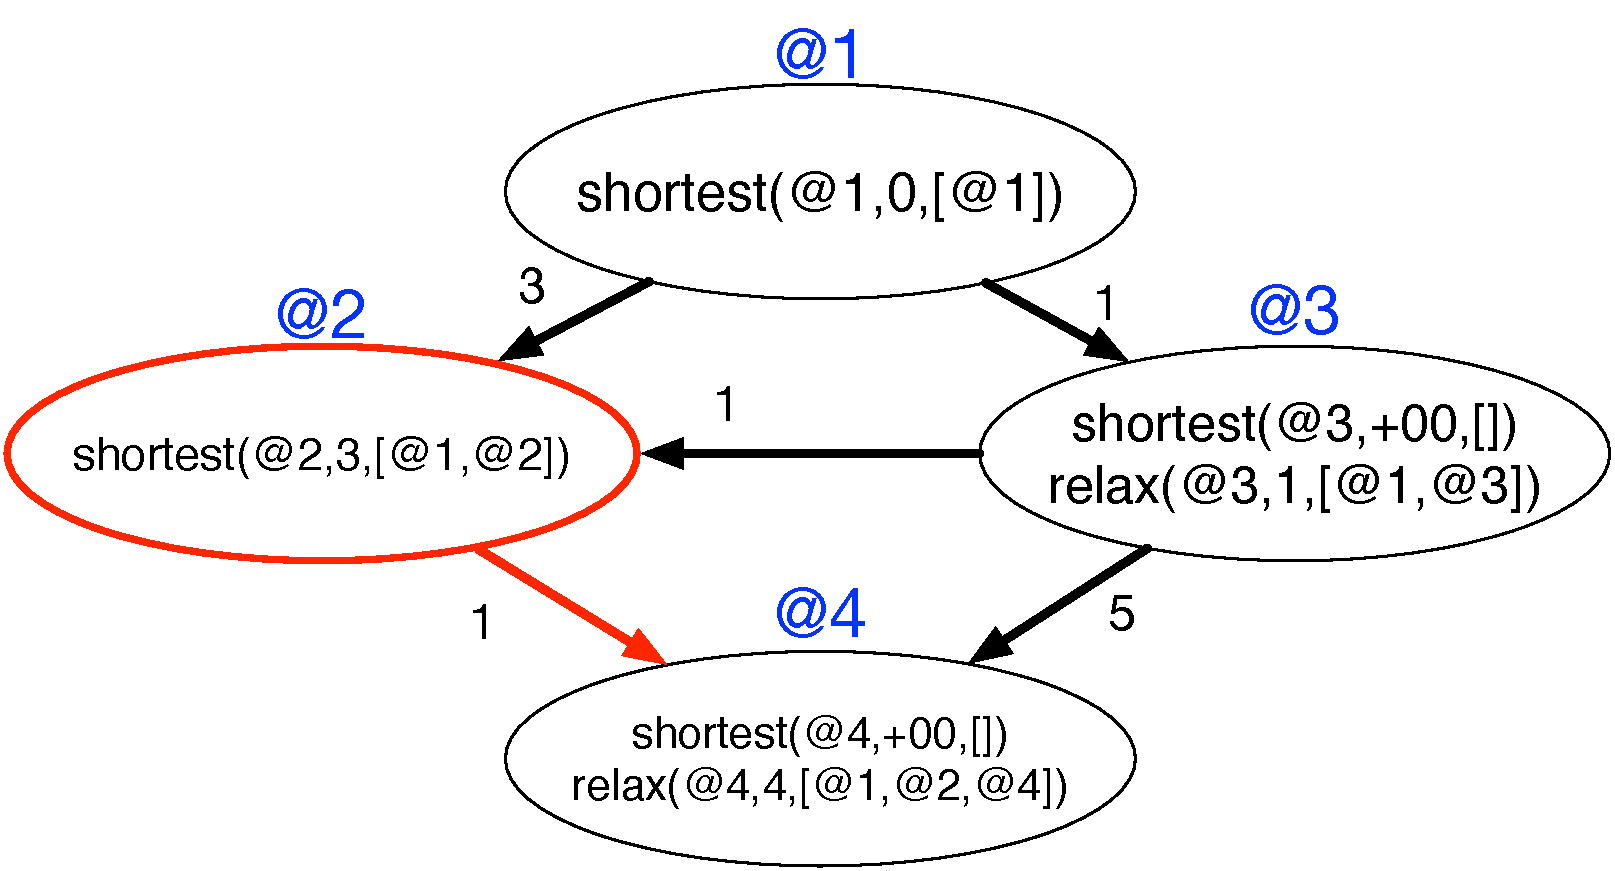
\includegraphics[width=0.32\textwidth]{figures/shortest3}}
  \hspace{0.02cm}
  \subfloat[]{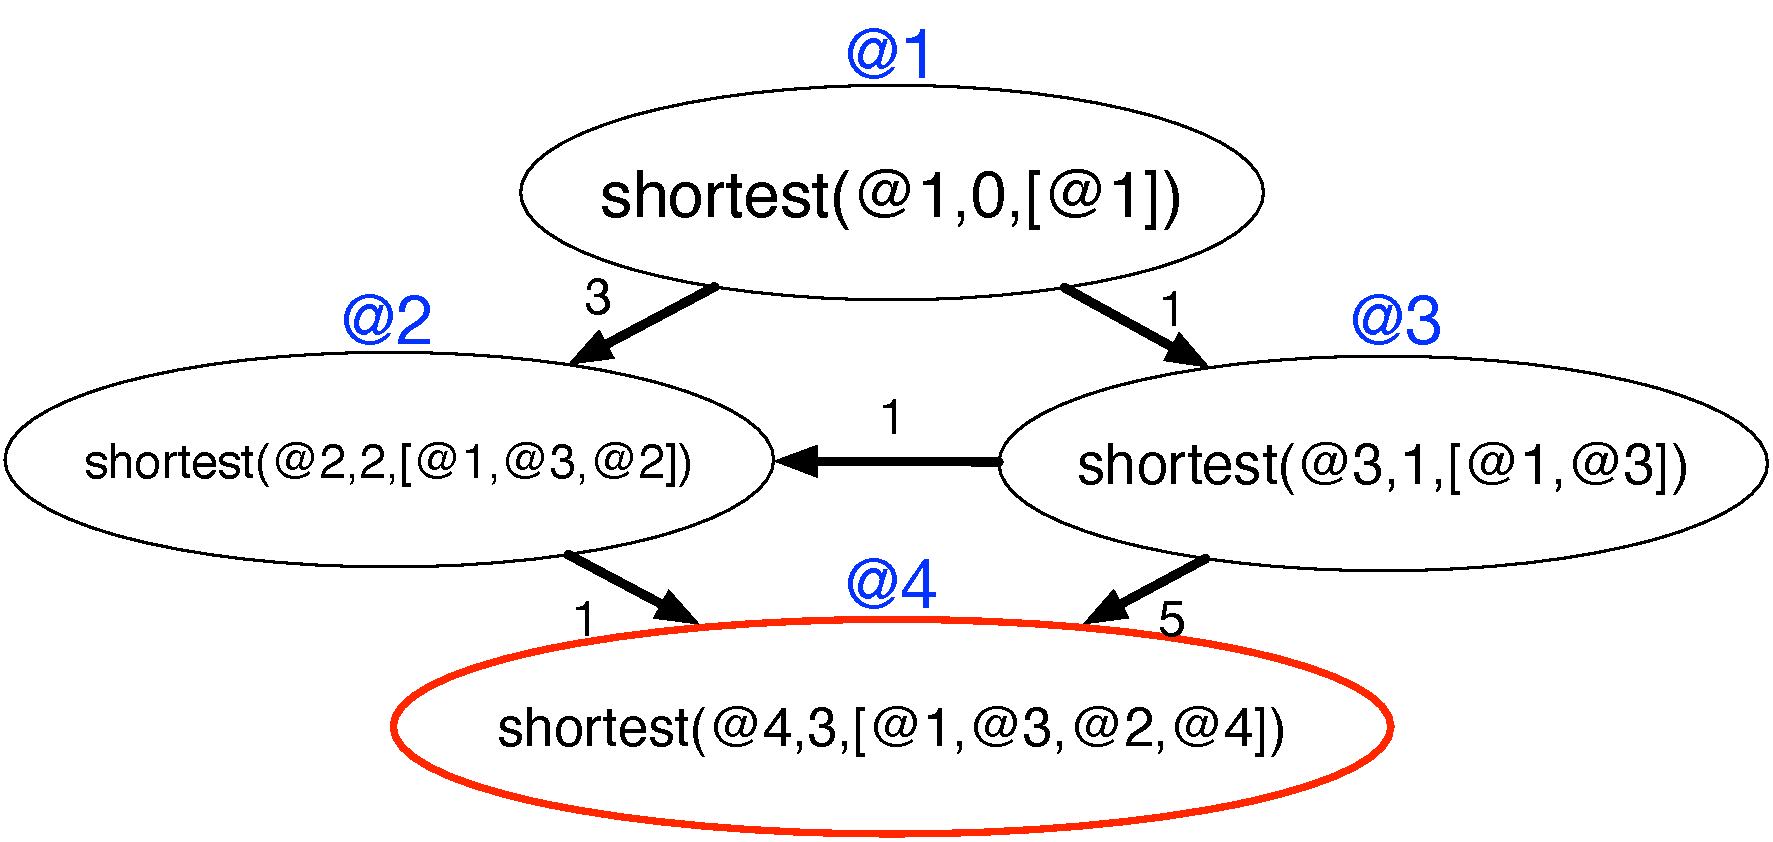
\includegraphics[width=0.32\textwidth]{figures/shortest8}}
\end{center}
\caption{Graphical representation of the SSSP program. (a) represents the
   program after propagating initial distance at node \mytt{@1}, followed by
   (b) where the first rule is applied in node \mytt{@2}. (c)
   represents the final state of the program, where all the shortest paths
   have been computed.}
\label{fig:shortest_path_program}
\end{figure}


\subsection{LM Syntax}

\begin{table}[h]
\centering
\begin{tabular}{ l l c l }
  Program & $Prog$ & $::=$ & $\Sigma, D$ \\
  List Of Rules & $\Sigma$ & $::=$ & $\cdot \; | \; \Sigma, R$\\
  Database & $D$ & $::=$ & $\Gamma; \Delta$ \\
  Rule & $R$ & $::=$ & $BE \lolli HE \; | \; \forall_{x}. R$ \\
  Body Expression & $BE$ & $::=$ & $L \; | \; P \; | \; C \; | \; BE, BE \; | \; \one$\\
  Head Expression & $HE$ & $::=$ & $L \; | \; P \; | \; HE, HE \; | \; EE \; |
  \; CE \; | \; AE \; | \; \one$\\
  
  Linear Fact & $L$ & $::=$ & $l(\hat{x})$\\
  Persistent Fact & $P$ & $::=$ & $\bang p(\hat{x})$\\
  Constraint & $C$ & $::=$ & $c(\hat{x})$ \\
  Selector Operation & $S$ & $::=$ & $\mathtt{min} \; | \; \mathtt{max} \; | \; \mathtt{random}$\\
  
  Comprehension & $CE$ & $::=$ & $\comprehension{\widehat{x}}{SB}{SH}$ \\

  Aggregate & $AE$ & $::=$ & $\aggregate{A}{y}{\widehat{x}}{SB}{SH_1}{SH_2}$ \\
  Aggregate Operation & $A$ & $::=$ & $\mathtt{min} \; | \; \mathtt{max} \; | \;
\mathtt{sum} \; | \; \mathtt{count} \; | \; \mathtt{collect}$ \\
  
  Sub-Body & $SB$ & $::=$ & $L \; | \; P \; | \; SB, SB \; | \; \exists_{x}. SB$\\
  Sub-Head & $SH$ & $::=$ & $L \; | \; P \; | \; SH, SH \; | \; \one$\\
  
  Known Linear Facts & $\Delta$ & $::=$ & $\cdot \; | \; \Delta, l(\hat{t})$ \\
  Known Persistent Facts & $\Gamma$ & $::=$ & $\cdot \; | \; \Gamma, \bang p(\hat{t})$ \\
\end{tabular}
\caption{Abstract syntax of LM.}\label{tbl:ast}
\end{table}

The abstract syntax for LM programs is presented in Table~\ref{tbl:ast}.  A LM
rule is written as $BE \lolli HE$ where $BE$ is the body and $HE$ is the head of
the rule. The body may contain linear ($L$) and persistent ($P$) \emph{fact
   expressions} and \emph{constraints} ($C$). Fact expressions instantiate facts
from the database and contain variables as arguments that may or may not be
bound to concrete values or to other variables.  Variables in the body of the
rule can also be used in the head when instantiating facts.  Constraints are
essential for matching rules since they represent database \emph{joins} and
database \emph{selects}.  While selects filter out possible combinations from
the database, body constraints ($C$) further restrict combinations by acting as
guards using small variables from fact expressions.  Constraints use a small
functional language that includes mathematical operations, boolean operations,
external functions and literal values.

The head of a rule, $HE$, contains linear ($L$) and persistent ($P$) \emph{fact
   templates} which are uninstantiated facts and will derive new facts. The head
can also have \emph{comprehensions} ($CE$) and \emph{aggregates} ($AE$). All
those expressions may use all the variables instantiated in the body.

Comprehensions are similar to the functional programming construct of the same
name.  Comprehensions are sub-rules that are applied for all possible
combinations. In a comprehension $\comprehension{\widehat{x}}{SB}{SH}$,
$\widehat{x}$ is a list of variables, $SB$ is the body of the comprehension and
$SH$ is the head. The body $SB$ is used to generate all possible combinations
for the head $SH$, according to the facts in the database.  An example was shown
in Fig.~\ref{code:shortest_path_program} (lines 13-14), where \mytt{\bang
   edge(A, B, W)} facts are iterated over in order to derive \texttt{relax(A, D2
   + W, P2 ++ [B])} facts for each combination.

Aggregates build on top of comprehensions and allow the capture of values that
appear in each combination of the sub-rules. This list of values is then
combined using one operator into a single value and then used to derive a set of
fact expressions. In the abstract syntax
$\aggregate{A}{y}{\widehat{x}}{SB}{SH_1}{SH_2}$, $A$ is the aggregate operation,
$\widehat{x}$ is the list of variables introduced in $BE$ and $SH_1$ and $y$ is
the variable in the body $SB$ that represents the values to be aggregated using
$A$. Like comprehensions, we use $\widehat{x}$ to try all the combinations of
$SB$, but, in addition to deriving $SH_1$ for each combination, we aggregate the
values represented by $y$ into a new $y$ variable that is used inside the head
$SH_2$.  LM provides several aggregate operations, including the \texttt{min}
(minimum value), \texttt{max} (maximum value), \texttt{sum} (add all numbers),
\texttt{count} (count combinations) and \texttt{collect} (collect items into a
list). Consider, for example, the following rule:

\begin{Verbatim}[fontsize=\scriptsize]
const P = ... // number of nodes
const damp = 0.15.

update(A), pagerank(A, OldRank)
      -o [sum => V | B | neighbor-pagerank(A, B, V) |
            neighbor-pagerank(A, B, V) |
            pagerank(A, damp/P + (1.0 - damp) * V)].
\end{Verbatim}

The rule uses an aggregate to accumulate the sum of the neighbor's PageRank into
a single value \texttt{V}. This aggregate value is then assigned to a new
\texttt{pagerank} fact via the expression \texttt{damp/P + (1.0 - damp)*V},
where \texttt{V} is the result of adding all the \texttt{V} values in
\texttt{neighbor-pagerank(A, B, V)} facts.
